\chapter{语言处理器基本概}

\begin{center}
学而不思则罔,思而不学则怠!
\end{center}

\begin{flushright}
---孔子    
\end{flushright}

\section{机器语言与汇编语言}
本节主要介绍了机器语言与汇编语言:
\begin{itemize}
    \item 机器语言是可以由机器直接解释执行的语言,一般才用二进制形式\cite{complete}。
    \item 汇编语言一般是相对于机器语言更易理解的语言,但是又因不同的体系结构不同具有不
    同的指令集。
\end{itemize} 


\section{解释器与编译器}
本节主要介绍了解释器和编译器的区别:
\begin{itemize}
    \item 解释器根据程序中的算法执行运算。
    \item 编译器将某种语言写成的程序转换为另一种语言的程序。
\end{itemize}    
    
\section{开发语言处理器}
本节主要介绍语言处理器,综合了解释器和编译器的优点。

\section{语言处理器结构与本书框架}
语言处理器的基本结构,如图1.1所示,画出了语言处理器的基本处理结构,源程序通过词法分析进行
单词排列,然后经过语法分析生成一个抽象语法树,然后根据是编译器还是解释器执行不同的步骤,
如果是编译器则直接生成机器语言,如果是解释器则一边分析抽象语法树,一边输出执行结果。
\begin{figure}[hbtp]
\centering
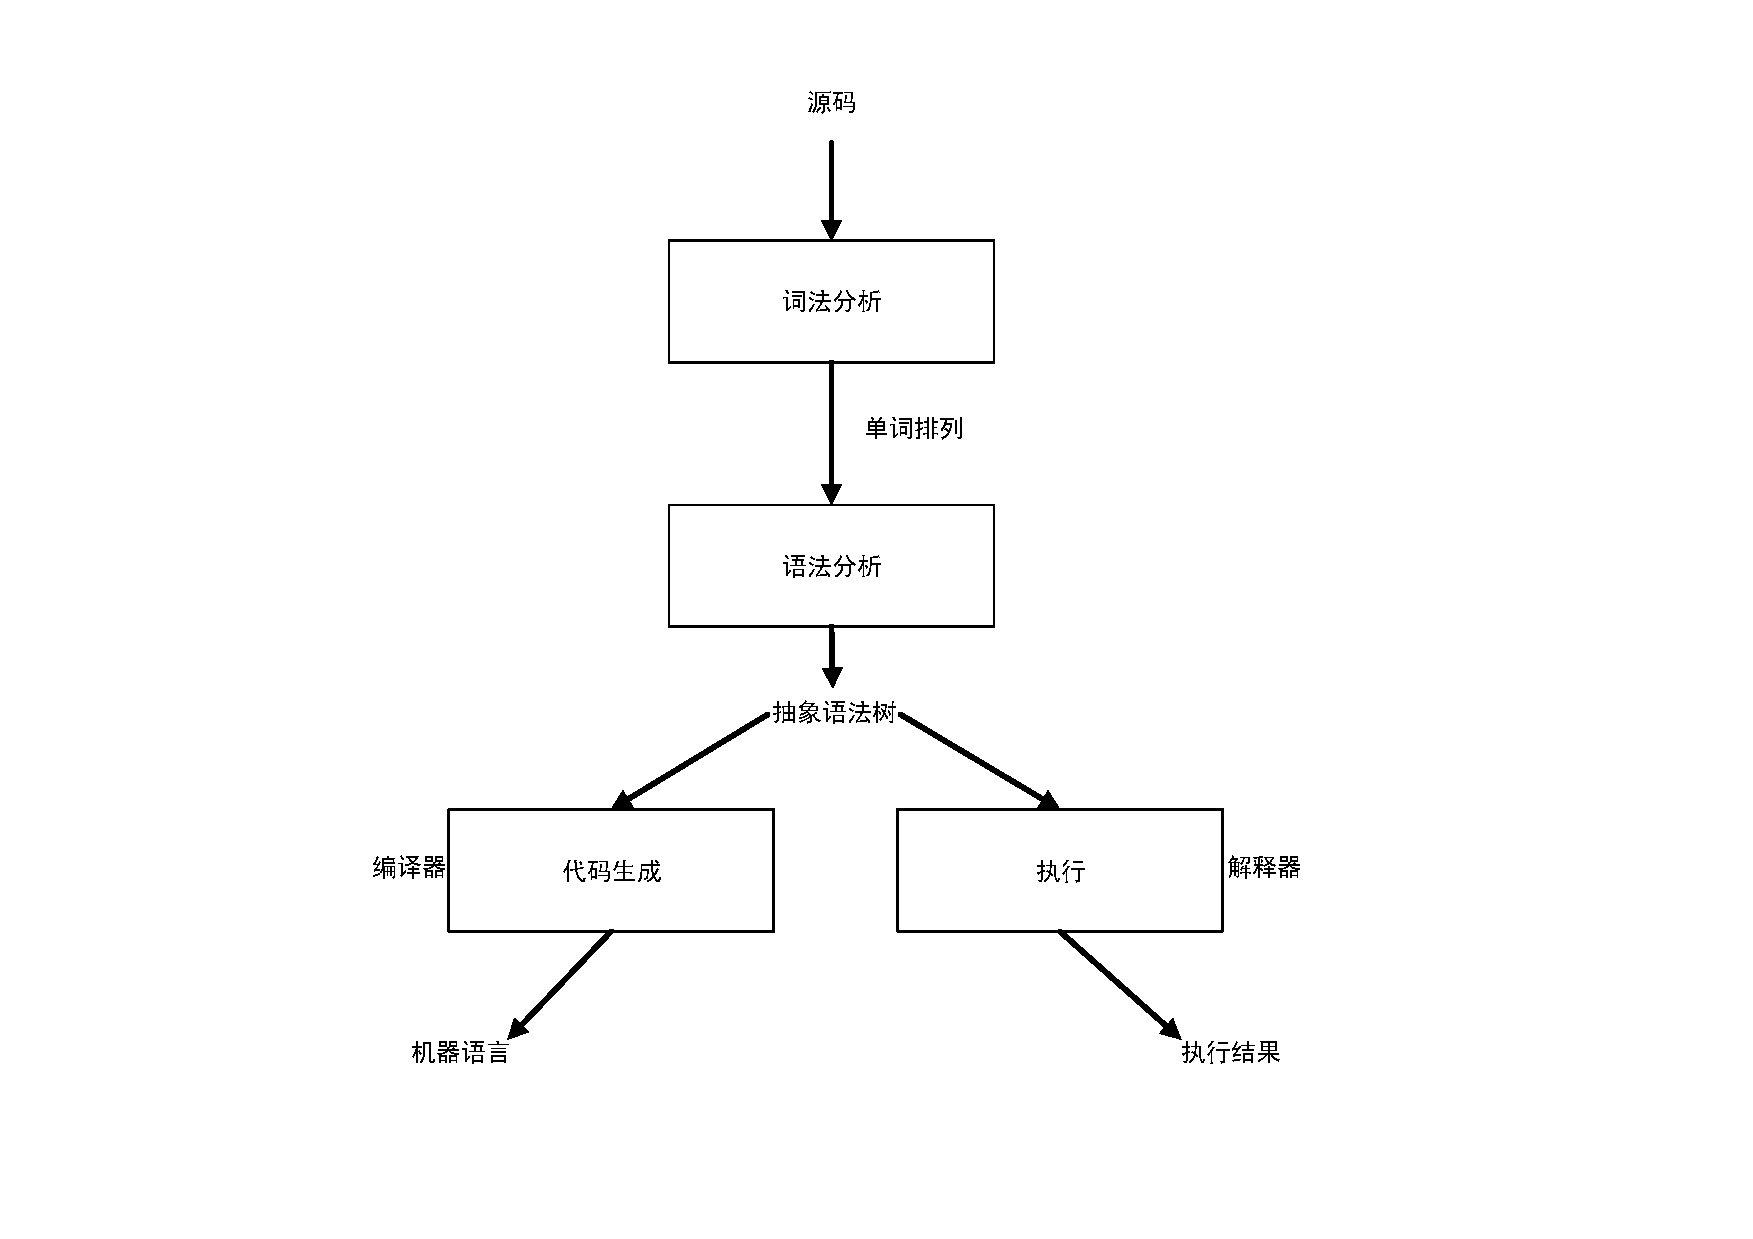
\includegraphics[width=1.0\textwidth]{construction.pdf}
\caption{语言处理器结构}
\end{figure}


无论是编译器还是解释器的结构都是大同小异的,第一步都是要先进行词法分析,由一长串字符分解
成为多个更小的字符串单元,然后执行语法分析,把单词排列成为抽象语法树,到此解释器与编译器
的行为都是一致的,在这之后编译器将转换为另外的语言,而解释器则将一边分析语法树一边执行。